\chapter{Hochschule Furtwangen}

\section{Profil \& Leitbild}

Die \gls{HFU} ist eine führende Hochschule in Deutschland und zeichnet sich durch Spitzenpositionen auf folgenden Gebieten aus:

\begin{itemize}
    \item Hohe Qualität und Innovation in der Lehre
    \item Praxisbezug durch Kooperation mit der Wirtschaft
    \item Internationale Kooperationen
    \item Angewandte Forschung
    \item Weiterbildung und lebenslanges Lernen
    \item Qualifikation und Motivation
    \item Soziale Verantwortung und Zukunftssicherung
\end{itemize}

\section{Zitate}
\blindtext \autocite{the_art_of_computer_programming}

\section{Mathematische Darstellungen}

\blindmathpaper

\section{Tabellen}
Siehe \tablename\ \ref{tab:example}

\begin{table}[H]
    \centering
    \begin{tabular}{@{}lll@{}}
        \toprule
        Spalte 1 & Spalte 2 & Spalte 3 \\
        foo      & bar      & baz      \\
        \bottomrule
    \end{tabular}
    \caption{Beispieltabelle}
    \label{tab:example}
\end{table}

\section{Abbildungen}
\figurename\ \ref{fig:mips_architektur}

\begin{figure}[H]
    \centering
    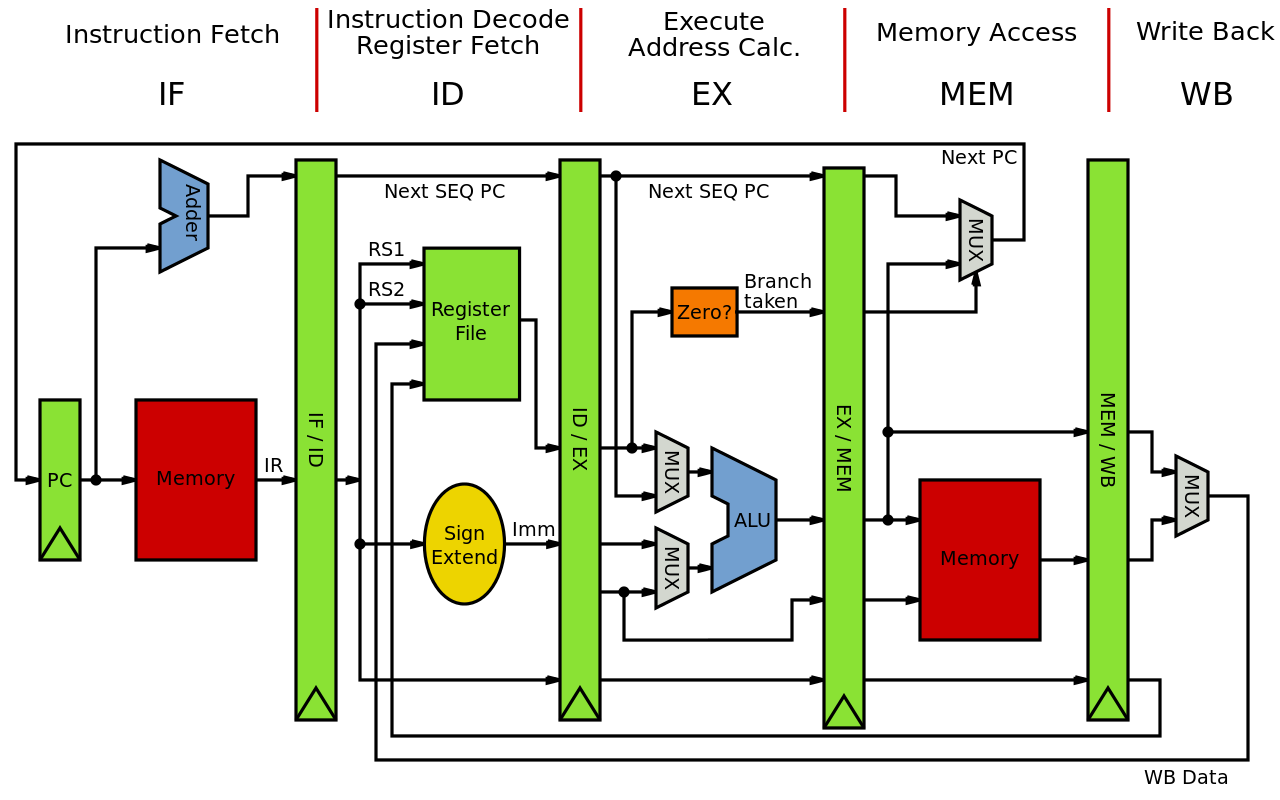
\includegraphics[width=1.0\textwidth]{medien/mips_architecture}
    \caption{MIPS Architektur}
    \label{fig:mips_architektur}
\end{figure}


\section{Listings}

\listingname\ \ref{listing:symfony_http_kernel}

\begin{code}
    \captionof{code}{HttpKernel.php}
    \label{listing:symfony_http_kernel}
    \begin{minted}[]{php}
    public function handle(Request $request, $type = HttpKernelInterface::MASTER_REQUEST, $catch = true)
    {
        $request->headers->set('X-Php-Ob-Level', ob_get_level());
        try {
            return $this->handleRaw($request, $type);
        } catch (\Exception $e) {
            if ($e instanceof RequestExceptionInterface) {
                $e = new BadRequestHttpException($e->getMessage(), $e);
            }
            if (false === $catch) {
                $this->finishRequest($request, $type);
                throw $e;
            }
            return $this->handleException($e, $request, $type);
        }
    }
    \end{minted}
\end{code}
